
\usepackage{fancyhdr}
\usepackage{lastpage}
\usepackage[utf8]{inputenc}

% Minted for syntax highliting
\usepackage{minted}
\usemintedstyle{tango}

% 
\usepackage[T1]{fontenc}
\usepackage{lmodern}

\usepackage{calc}
\usepackage{bytefield}

\usepackage{listings}
\usepackage{amsmath}

\usepackage{tikz}
\usetikzlibrary{automata,arrows,topaths,calc,positioning}
 
\usepackage{syntax}
\grammarindent=2cm


% Headers/footers styling
\pagestyle{fancy}
\fancyhf{}
\renewcommand{\headrulewidth}{0pt}

% Footer
\lfoot{ID1019}
\cfoot{KTH}
\rfoot{\thepage \hspace{1pt} / \pageref{LastPage}}

%\newcommand{\defaultpagestyle}{\thispagestyle{plain}}
\newcommand{\defaultpagestyle}{\thispagestyle{fancy}}



\title[ID1019 Morse coding]{Morse}


\author{Johan Montelius}
\institute{KTH}
\date{\semester}

\begin{document}



\begin{frame}
\titlepage
\end{frame}


\begin{frame}

  \begin{figure}
    \center
    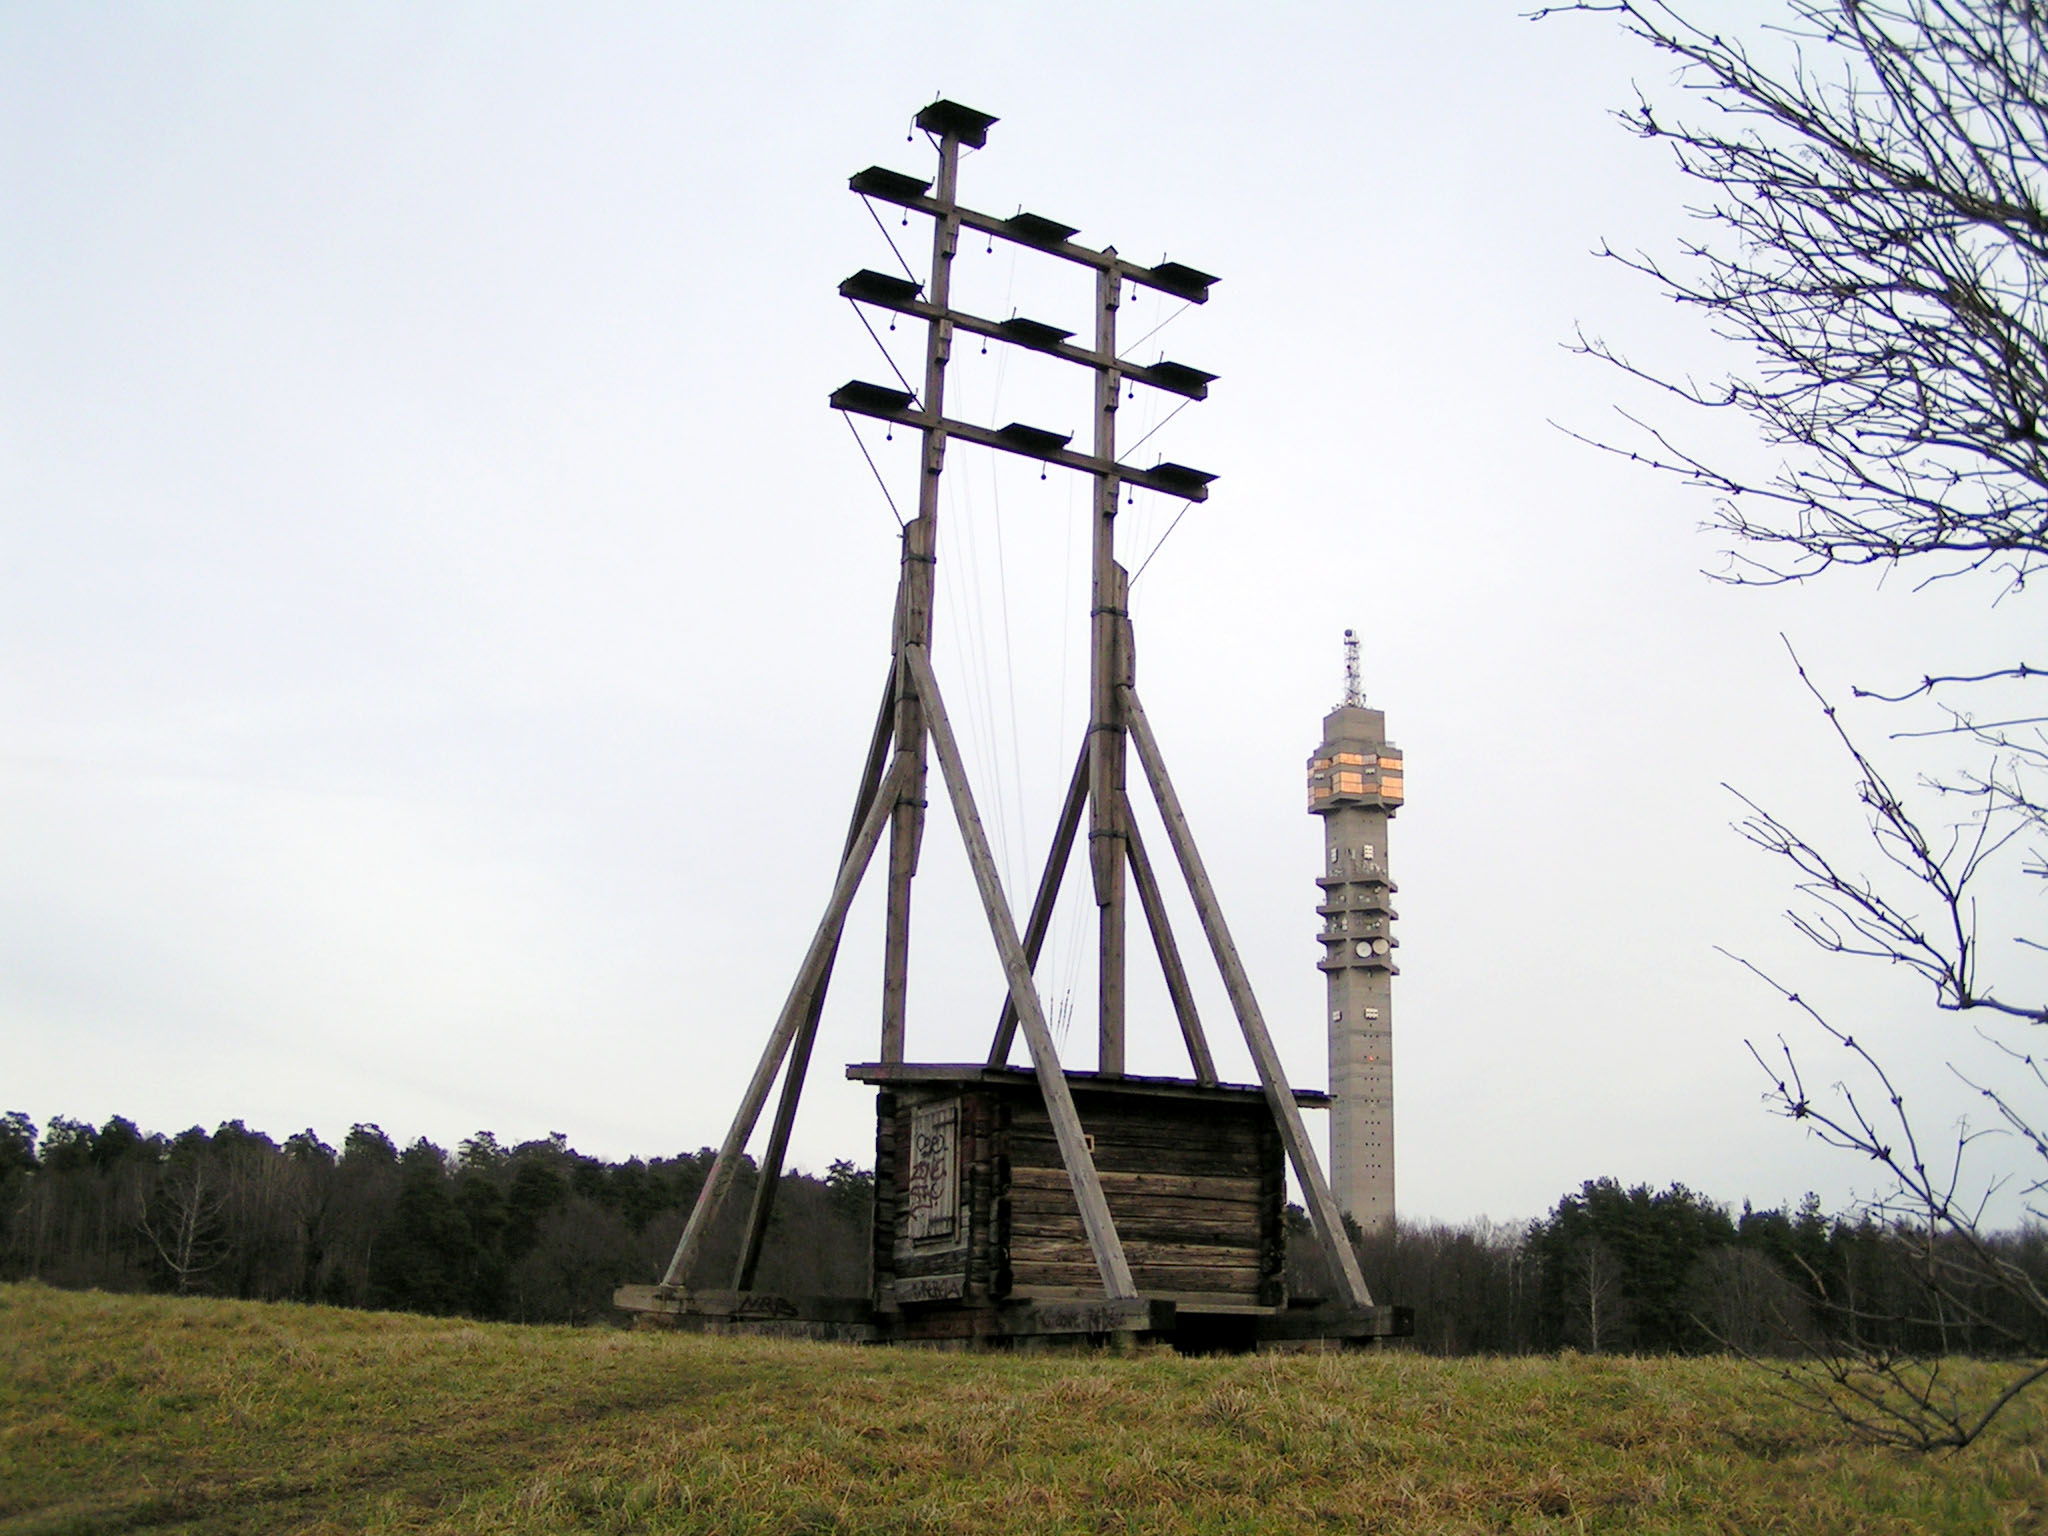
\includegraphics[scale=0.1]{gardet.jpg}
  \end{figure}

  \vspace{10pt}\pause
  {\em Abraham Niclas Edelcrantz: 1794, optical signaling, reconstruction on Gärdet}
  
\end{frame}


\begin{frame}

  \begin{figure}
    \center
    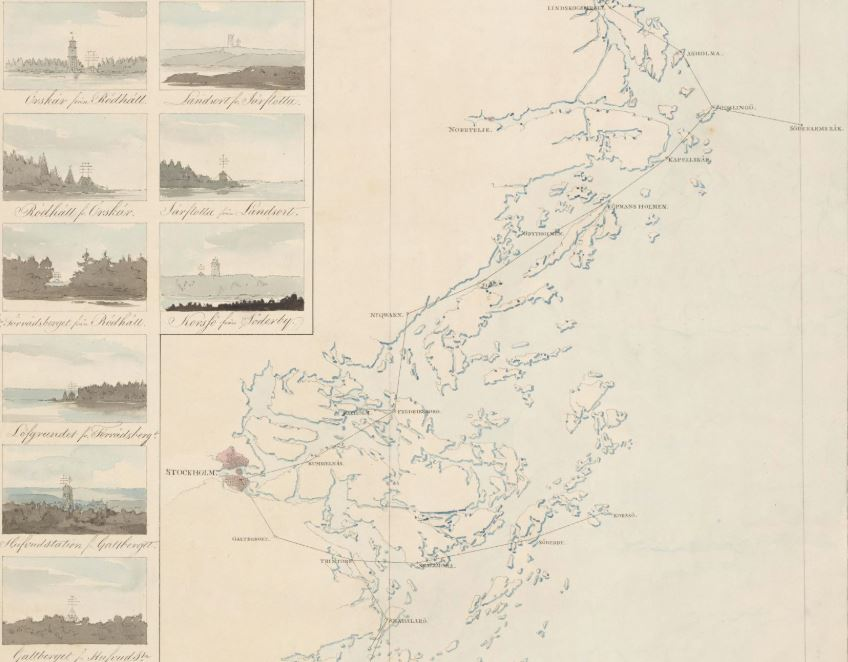
\includegraphics[scale=0.4]{stockholm.jpg}
  \end{figure}

  \vspace{10pt}\pause
  {\em Stockholm archipelago optical network: latency Sanhamn-Stockholm 10 min, 12 symbols/minute}
  
\end{frame}


\begin{frame}

  \begin{figure}
    \center
    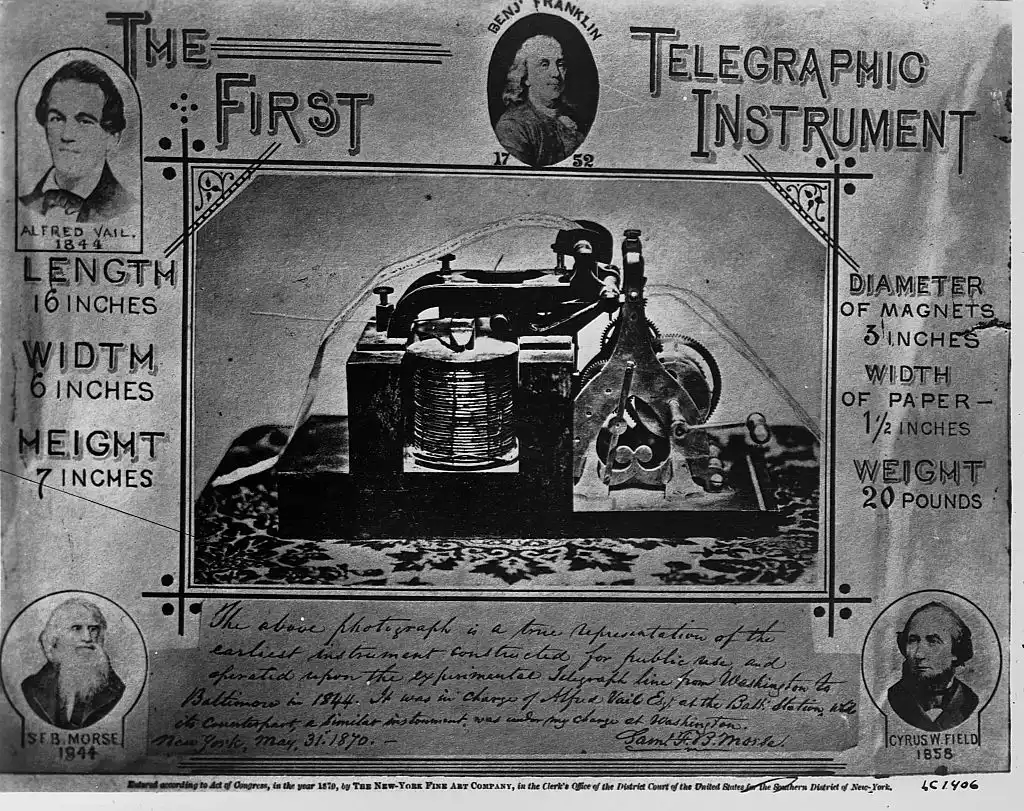
\includegraphics[scale=0.2]{morse.png}

  \end{figure}

  \vspace{10pt}\pause  
  {\em Samuel Morse - first telegraphic message in 1837, first telegraphic line 1844 Washington - Baltimore}
\end{frame}


\begin{frame}{the Morse alphabet}

  \begin{figure}
    \center
    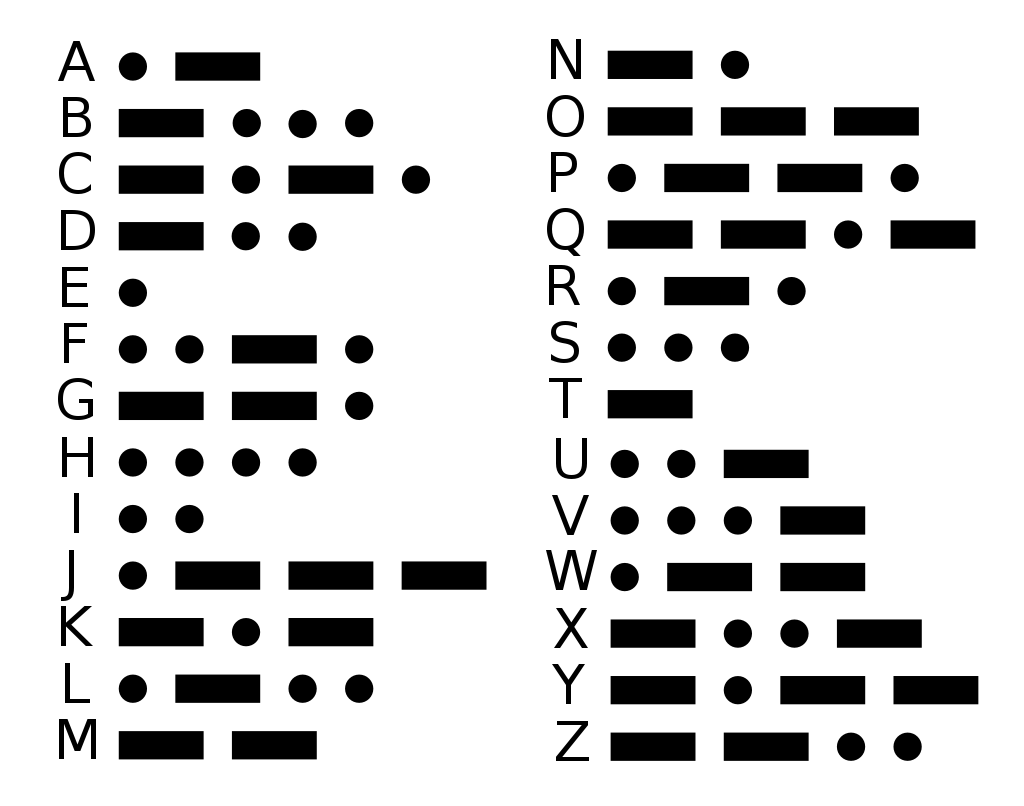
\includegraphics[scale=0.2]{code.png}

  \end{figure}

  \vspace{10pt}\pause  
  {\em The international Morse alphabet (national might differ)}

\end{frame}

\begin{frame}{Telegraphic network}
  \begin{figure}
    \center
    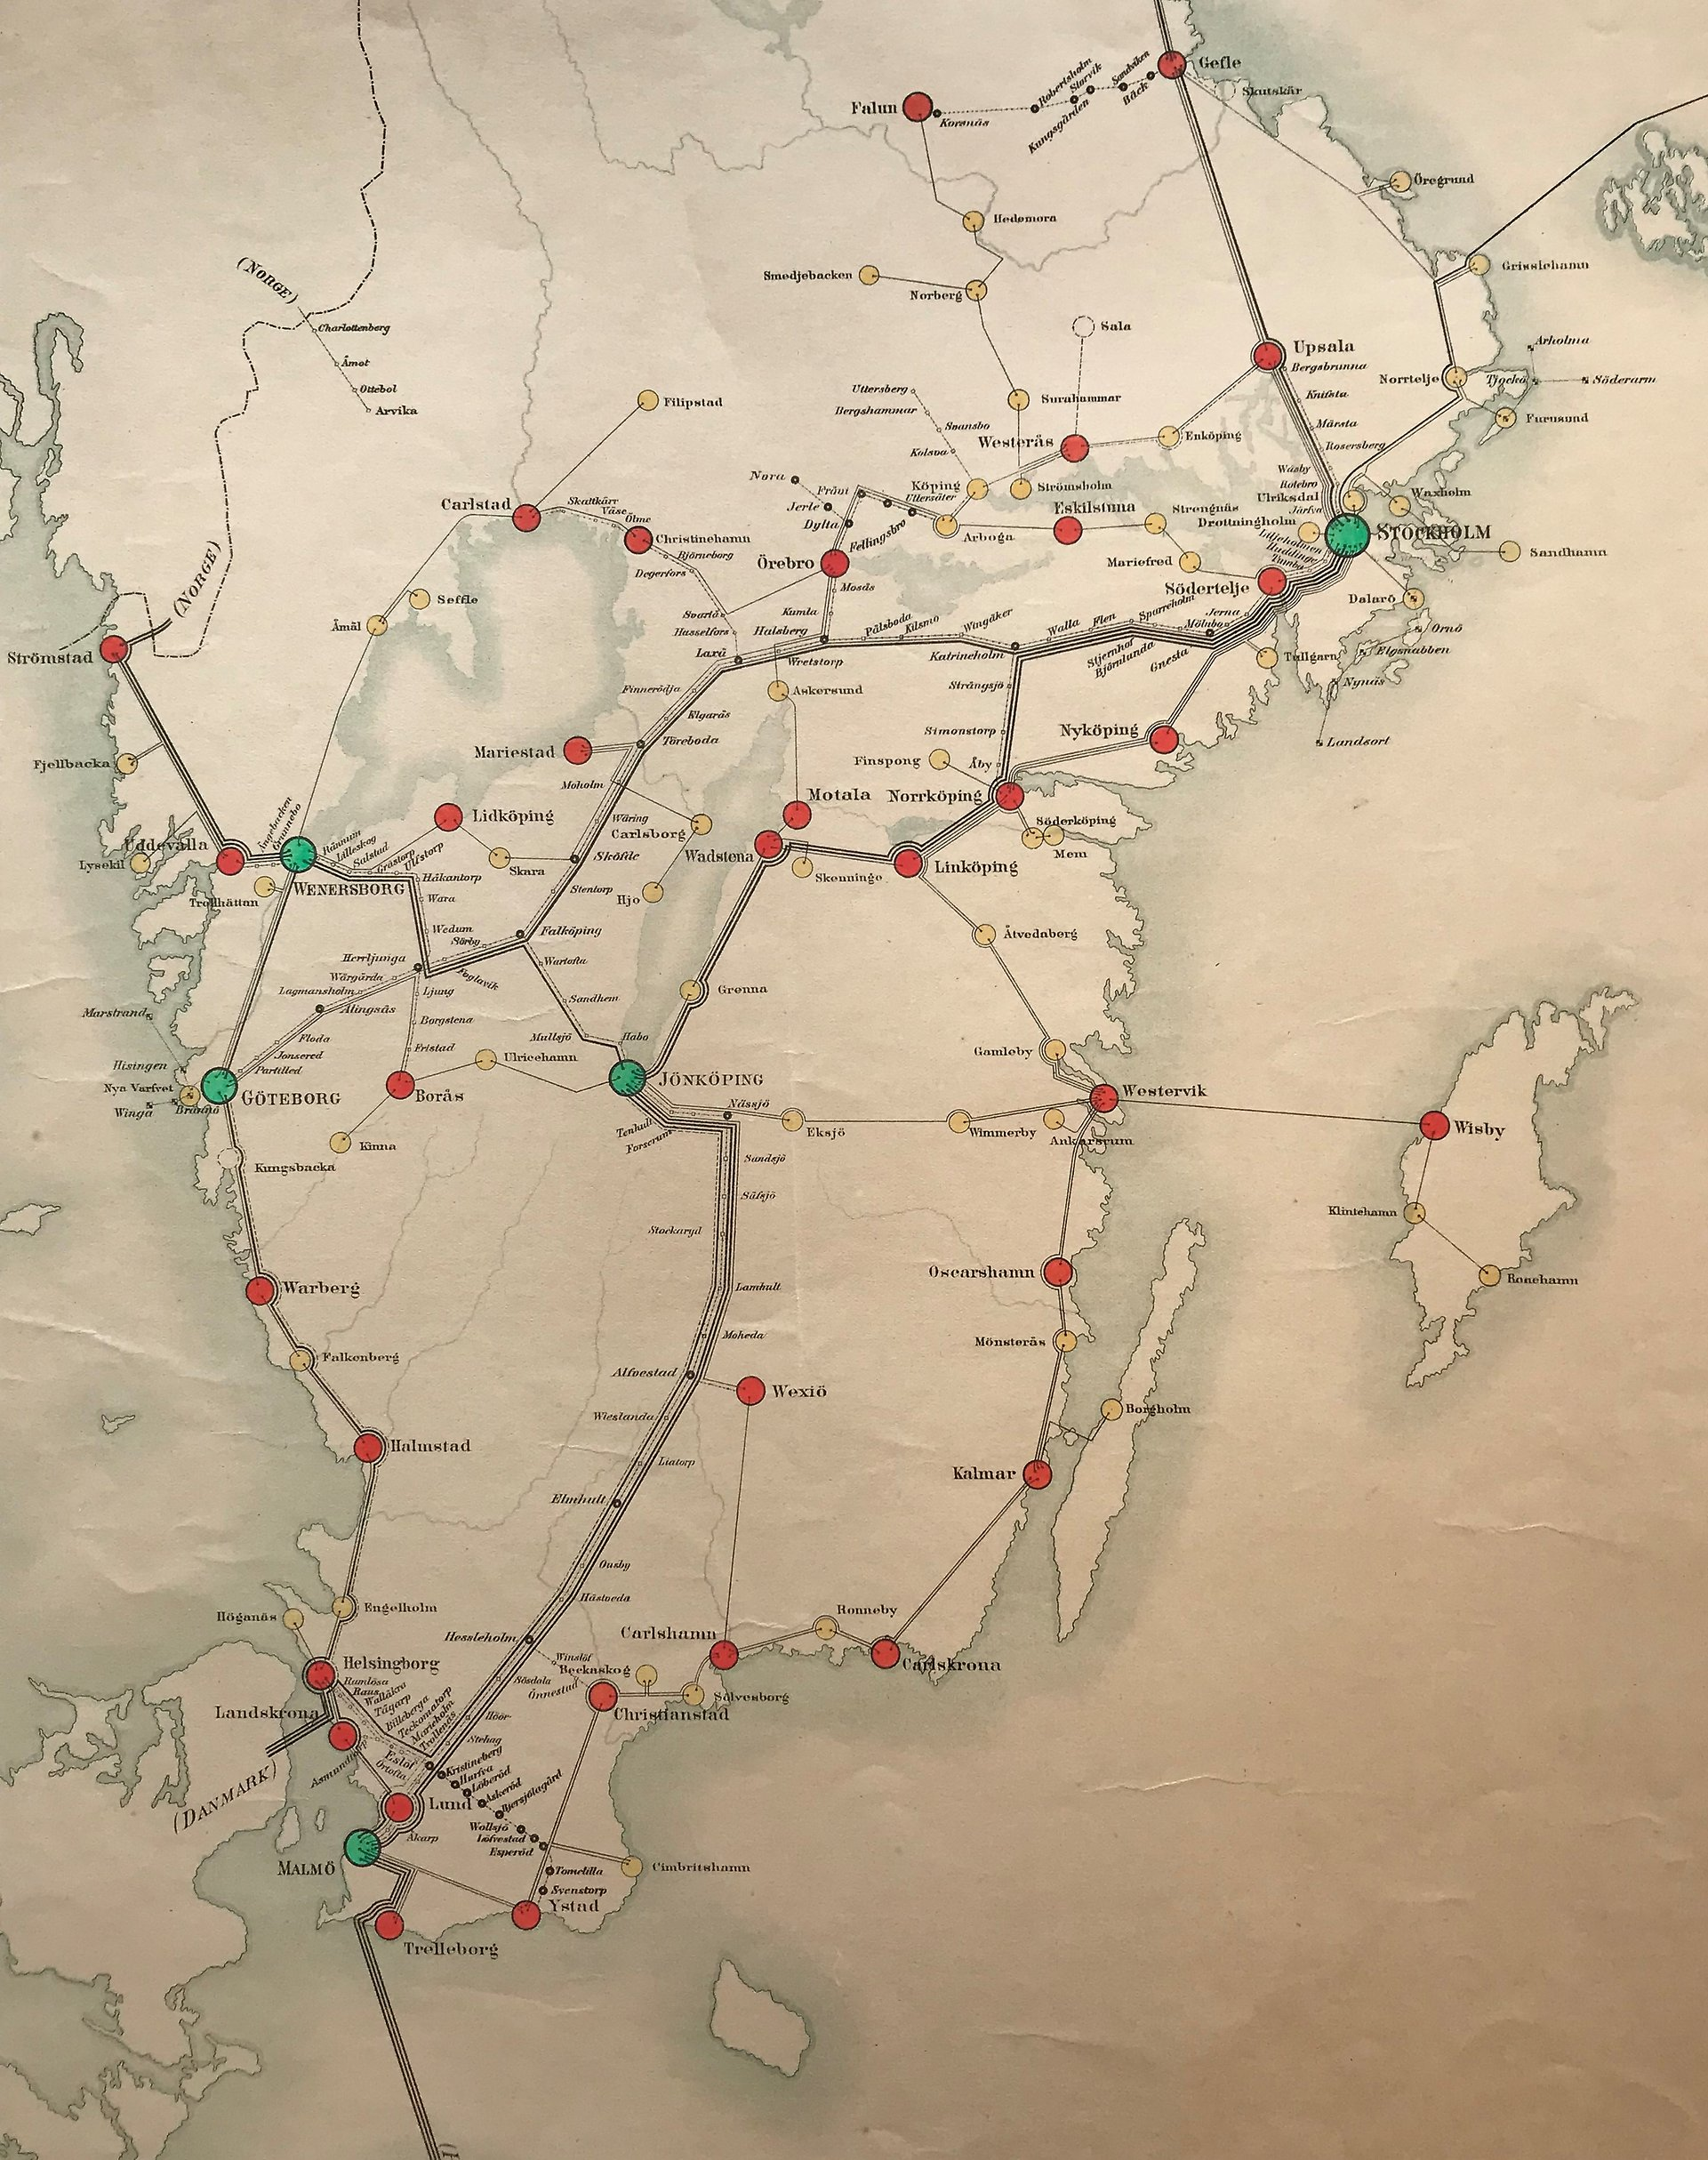
\includegraphics[scale=0.08]{sweden.jpg}

  \end{figure}

  \vspace{10pt}\pause  
  {\em Sweden 1870: larger cities connected.}
  
\end{frame}


\begin{frame}{WWII}

  \begin{figure}
    \center
    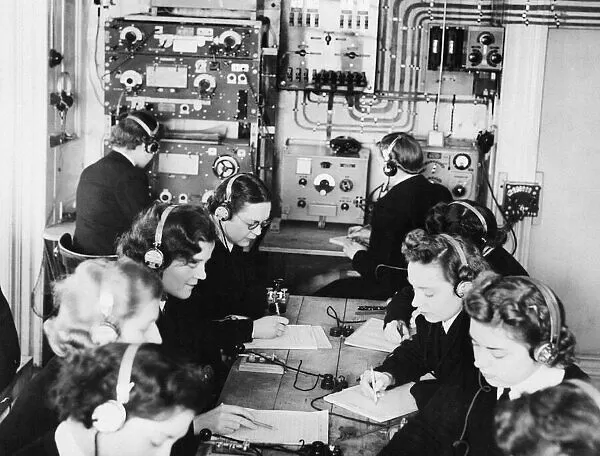
\includegraphics[scale=0.4]{women.png}

  \end{figure}

  \vspace{10pt}\pause  
  {\em Increased usage with the spread of radio communication, 60 characters/minute.}

\end{frame}


\begin{frame}{Your task}

  \begin{itemize}
  \item implement an encoder with atmost $O(n*lg(k)*c)$ time complexity:
    \begin{itemize}
     \item $n$ length of message
     \item $k$ number of characters in the alphabet
     \item $c$ average length of Morse code
     \item the encoder should not use more stack space then the length of the morse codes
     \end{itemize}

   \item encode your name: 'johan'  is '.--- --- .... .- -. '
   \item implement a decoder with at most $O(m)$ time complexity
     \begin{itemize}
     \item $m$ length of encoded message
     \end{itemize}
     \item decode two intercepted messages
   \end{itemize}
  
\end{frame}


\end{document}



